\documentclass[UTF8,fontset=windows,a4paper,12pt]{ctexart}

\usepackage{geometry}
\usepackage{graphicx}
\usepackage{booktabs}
\usepackage{tabularx}
\usepackage{longtable}
\usepackage{array}
\usepackage{float}
\usepackage{caption}
\usepackage{subcaption}
\usepackage{xcolor}
\usepackage{listings}
\usepackage{hyperref}
\usepackage{fancyhdr}
\usepackage{lastpage}
\usepackage{enumitem}
\usepackage{amsmath}
\usepackage{xurl}

\geometry{left=2.6cm,right=2.6cm,top=2.6cm,bottom=2.6cm}
\graphicspath{{assets/}}
\hypersetup{
  colorlinks=true,
  linkcolor=black,
  urlcolor=blue,
  citecolor=black
}

\pagestyle{fancy}
\fancyhf{}
\lhead{实验二 MCU 基础原理}
\rhead{罗丹 2251801014}
\cfoot{\thepage/\pageref{LastPage}}
\setlength{\headheight}{15pt}
\setlength{\parindent}{2em}
\setlength{\parskip}{0.35em}
\renewcommand{\arraystretch}{1.18}
\captionsetup{font=small,labelfont=bf}

\definecolor{codebg}{RGB}{247,248,250}
\definecolor{codeframe}{RGB}{220,224,230}
\definecolor{keywordblue}{RGB}{0,92,175}
\definecolor{commentgreen}{RGB}{72,132,72}
\lstdefinestyle{reportcode}{
  backgroundcolor=\color{codebg},
  frame=single,
  rulecolor=\color{codeframe},
  basicstyle=\ttfamily\small,
  keywordstyle=\color{keywordblue}\bfseries,
  commentstyle=\color{commentgreen},
  stringstyle=\color{purple},
  numbers=left,
  numberstyle=\tiny\color{gray},
  breaklines=true,
  columns=fullflexible,
  tabsize=2,
  showstringspaces=false,
  keepspaces=true
}
\lstset{style=reportcode}

\newcolumntype{Y}{>{\raggedright\arraybackslash}X}
\newcolumntype{R}{>{\raggedleft\arraybackslash}p{2.2cm}}

\begin{document}

\begin{titlepage}
\thispagestyle{empty}
\centering
\vspace*{1.45cm}

{\zihao{2}\bfseries 传感器与检测技术实验报告\par}

\vspace{2.15cm}

{\zihao{2}\bfseries 实验二：\quad MCU 基础原理\par}

\vspace{2.65cm}

{\zihao{-4}
\begin{tabular}{r@{\quad}l}
课程名称： & 传感器与检测技术 \\
\\[-0.15cm]
实验对象： & ESP32-S3 开发板 \\
\\[-0.15cm]
开发方式： & MicroPython + ESP-IDF/PlatformIO 补测 \\
\\[-0.15cm]
姓\hspace{2em}名： & 罗丹 \\
\\[-0.15cm]
学\hspace{2em}号： & 2251801014 \\
\\[-0.15cm]
GitHub： & \url{https://github.com/gf-be/ESP32_course} \\
\\[-0.15cm]
日\hspace{2em}期： & 2026 年 6 月 1 日 \\
\end{tabular}
\par}

\vfill
{\zihao{4} 福建理工大学\par}
\vspace*{0.85cm}
\end{titlepage}

\setcounter{page}{1}
\tableofcontents
\newpage

\section{摘要}

本实验基于 ESP32-S3 开发板完成 GPIO 输出、PWM、ADC、定时器中断、GPIO 外部中断、ADC DMA 双缓冲和板端时间戳测量。实验主要采用板内外设回环方式完成验证：GPIO5 输出 PWM 或测试脉冲，GPIO4 用作 ADC 采集输入；ESP-IDF 中断优先级补测中，GPIO7 输出 1 kHz 边沿，GPIO6 作为外部中断输入。

实验结果表明，1 kHz 定时器中断采集的 CPU 占用估计约为 8.494\%，明显低于忙等待查询方式；ESP-IDF 连续 ADC DMA 在 50 kHz 目标采样下实测 49997.0 Hz，CPU 占用约为 0.497\%；MicroPython 层 10000 次 GPIO 中断响应平均延迟约为 $29.723~\mu s$，jitter 标准差约为 $2.241~\mu s$；ESP-IDF 层 Level 1 与 Level 3 GPIO 中断平均延迟均约为 $3.500~\mu s$。

需要说明的是，标准 MicroPython 固件没有暴露 ESP32 ADC DMA 双缓冲接口，因此 DMA 双缓冲和不同中断优先级对比使用 ESP-IDF/PlatformIO 工程补测完成；MicroPython 部分保留 GPIO、PWM、ADC、定时器、中断和 1 小时时间戳的原始实测数据。

\section{实验目的与要求}

\begin{enumerate}[label=\arabic*.]
  \item 掌握微控制器 GPIO、PWM、ADC、定时器和外部中断的驱动开发方法。
  \item 理解 DMA 双缓冲工作原理，掌握高带宽数据采集的工程实现方式。
  \item 掌握嵌入式系统实时性指标测量方法，包括中断响应延迟、jitter 和时间戳精度。
  \item 理解实时性对系统的影响，建立微秒级工程精度意识。
\end{enumerate}

\section{实验环境与连接方式}

\begin{table}[H]
\centering
\caption{实验环境与引脚分配}
\begin{tabularx}{\textwidth}{lY}
\toprule
项目 & 内容 \\
\midrule
主机系统 & Windows \\
开发语言 & MicroPython, ESP-IDF C \\
开发板 & ESP32-S3 \\
板载 LED & GPIO48, NeoPixel RGB \\
PWM 输出 & GPIO5 \\
ADC 输入 & GPIO4 \\
中断测试 & MicroPython GPIO5 自触发 IRQ；ESP-IDF GPIO7 到 GPIO6 回环 \\
时间戳 & \texttt{time.ticks\_ms()}, \texttt{time.ticks\_us()} 与 PC 时间对比 \\
\bottomrule
\end{tabularx}
\end{table}

板内回环连接为 GPIO5 到 GPIO4，用于验证 PWM 输出和 ADC 采集；ESP-IDF 中断优先级补测连接为 GPIO7 到 GPIO6，由 GPIO7 输出 1 kHz 方波，GPIO6 配置为外部中断输入。由于现场没有独立信号发生器，本实验将“外部 1 kHz 方波触发”用同板 GPIO 方波替代，触发路径仍经过 GPIO 输入与中断模块。

\section{基础外设驱动实验}

\subsection{GPIO 输出与板载 RGB LED}

ESP32-S3 开发板板载 RGB LED 连接到 GPIO48，使用 NeoPixel 驱动完成输出验证。程序先控制红色 LED 闪烁，再进行蓝色亮度渐变，从而同时验证 GPIO 输出与类 PWM 亮度控制效果。

\begin{lstlisting}[language=Python,caption={板载 RGB LED 输出控制核心代码}]
def rgb_set(r, g, b):
    try:
        import neopixel
        np = neopixel.NeoPixel(machine.Pin(RGB_PIN, machine.Pin.OUT), 1)
        np[0] = (r, g, b)
        np.write()
        return True
    except Exception as exc:
        print("# rgb_unavailable,%s" % exc)
        return False

def run_board_rgb():
    ok = rgb_set(0, 0, 0)
    if not ok:
        return
    for _ in range(3):
        rgb_set(40, 0, 0)
        time.sleep_ms(200)
        rgb_set(0, 0, 0)
        time.sleep_ms(200)
\end{lstlisting}

运行结果为 GPIO48 板载 RGB LED 完成 3 次红色闪烁，并完成蓝色亮度渐变，说明 GPIO 输出控制正常。

\subsection{PWM 输出与 ADC 回环采集}

PWM 使用 GPIO5 输出 1 kHz 波形，并回接到 GPIO4 进行 ADC 采集。由于本实验直接采集 PWM 数字波形，没有增加 RC 低通滤波，因此单次 ADC 值主要表现为接近 0 V 或 3.3 V；统计均值和高电平采样比例可以反映占空比变化。

\begin{lstlisting}[language=Python,caption={PWM 输出核心代码}]
def run_external_pwm():
    pin = machine.Pin(PWM_PIN, machine.Pin.OUT)
    pwm = machine.PWM(pin, freq=1000, duty_u16=0)
    for _ in range(2):
        for duty in range(0, 65536, 2048):
            pwm.duty_u16(duty)
            time.sleep_ms(10)
        for duty in range(65535, -1, -2048):
            pwm.duty_u16(duty)
            time.sleep_ms(10)
    pwm.deinit()
    pin.off()
\end{lstlisting}

\begin{table}[H]
\centering
\caption{PWM 到 ADC 回环统计结果}
\begin{tabular}{rrrrr}
\toprule
PWM 占空比 & 样本数 & ADC 均值 & 估算电压 & 高电平采样比例 \\
\midrule
0\% & 1500 & 0.00 & 0.0000 V & 0.00\% \\
25\% & 1500 & 16122.35 & 0.8118 V & 24.60\% \\
50\% & 1500 & 32680.82 & 1.6456 V & 49.87\% \\
75\% & 1500 & 48932.94 & 2.4640 V & 74.67\% \\
100\% & 1500 & 65535.00 & 3.3000 V & 100.00\% \\
\bottomrule
\end{tabular}
\end{table}

\begin{figure}[H]
  \centering
  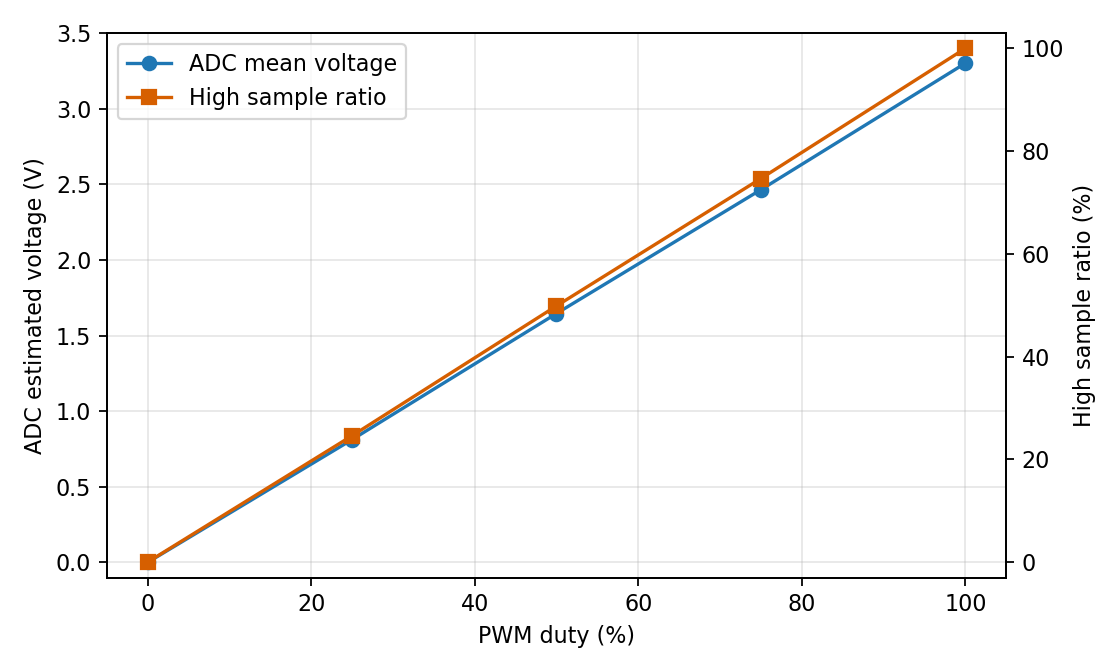
\includegraphics[width=0.82\textwidth]{pwm_adc_loopback_stats.png}
  \caption{PWM 占空比与 ADC 采样统计}
\end{figure}

从图表可见，占空比 25\%、50\%、75\% 时，高电平采样比例分别约为 24.60\%、49.87\%、74.67\%，与设定值基本一致，说明 PWM 输出与 ADC 采集链路有效。

\section{定时器中断与 DMA 双缓冲}

\subsection{查询方式与定时器中断对比}

MicroPython 测试脚本 \texttt{code/02\_polling\_vs\_timer\_adc.py} 对比了最大速率查询方式、1 kHz 忙等待查询方式和 1 kHz 定时器中断方式。定时器中断方式在回调函数中读取 ADC，并记录相邻采样时间间隔和服务时间。

\begin{lstlisting}[language=Python,caption={定时器中断 ADC 采样核心代码}]
def timer_cb(timer):
    global timer_count, timer_last
    t0 = time.ticks_us()
    if timer_count == 0:
        timer_last = t0
    if timer_count < TIMER_N:
        timer_values[timer_count] = adc_read()
        timer_dt[timer_count] = time.ticks_diff(t0, timer_last)
        timer_last = t0
        timer_service[timer_count] = time.ticks_diff(time.ticks_us(), t0)
        timer_count += 1
\end{lstlisting}

\subsection{DMA 双缓冲补测}

ESP-IDF 补测工程位于 \texttt{code/espidf\_dma\_irq/}。程序使用 ADC continuous driver，从硬件 DMA 环形缓冲区批量取样，并按帧统计吞吐量、处理时间和 CPU 占用。由于 MicroPython 标准固件未暴露 ESP32 ADC DMA 双缓冲接口，DMA 部分使用 ESP-IDF C 工程实现更符合底层外设能力。

\begin{table}[H]
\centering
\caption{采集方式性能对比}
\begin{tabularx}{\textwidth}{lrrrY}
\toprule
采集方式 & 最大或目标采样率 & CPU 占用率 & 丢包率 & 适用场景 \\
\midrule
查询方式 & 13586.7 Hz & 100.0\% & 0.000\% & 极简单低速采样或极限轮询测试 \\
1 kHz 忙等待查询 & 1000.3 Hz & 100.0\% & 0.000\% & 需要固定频率但不能释放 CPU 的临时测试 \\
定时器中断 & 999.0 Hz & 8.494\% & 0.000\% & 周期稳定、CPU 可执行其他任务的采集 \\
ESP-IDF 查询方式 & 18373.7 Hz & 100.000\% & 0.000\% & C 层阻塞轮询基准 \\
DMA 双缓冲 & 49997.0 Hz & 0.497\% & 0.000\% & ESP-IDF 连续 ADC DMA，高带宽批量采集 \\
\bottomrule
\end{tabularx}
\end{table}

\begin{figure}[H]
  \centering
  \begin{subfigure}{0.32\textwidth}
    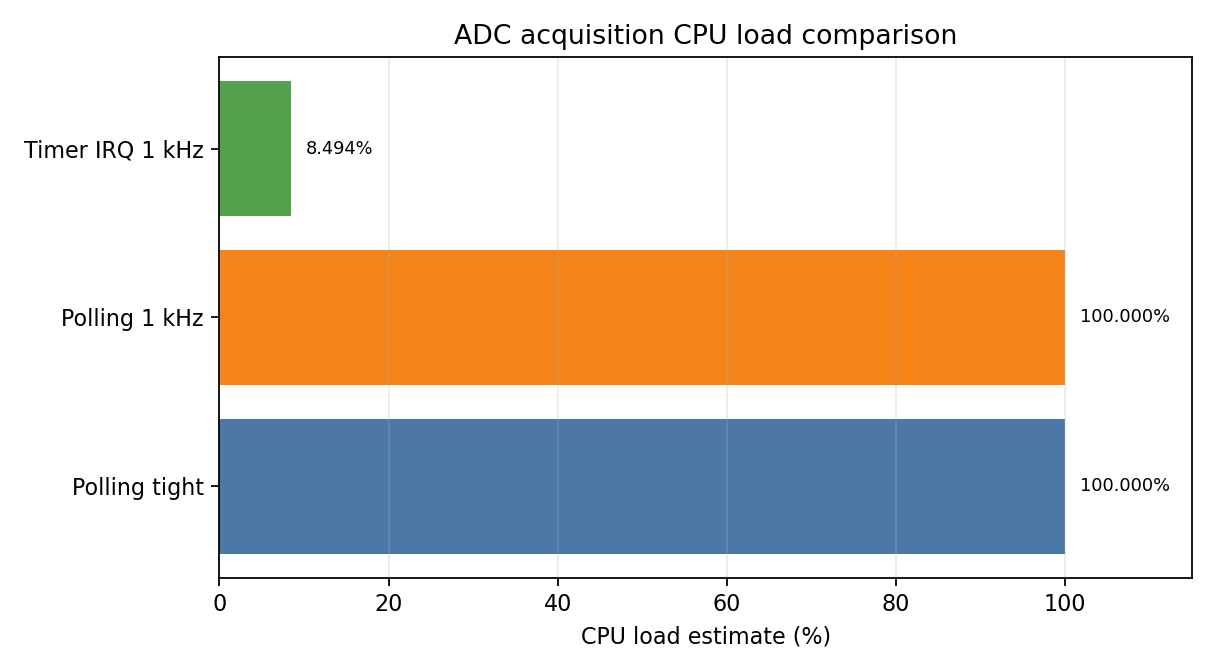
\includegraphics[width=\textwidth]{adc_cpu_load_comparison.png}
    \caption{MicroPython CPU 占用}
  \end{subfigure}
  \hfill
  \begin{subfigure}{0.32\textwidth}
    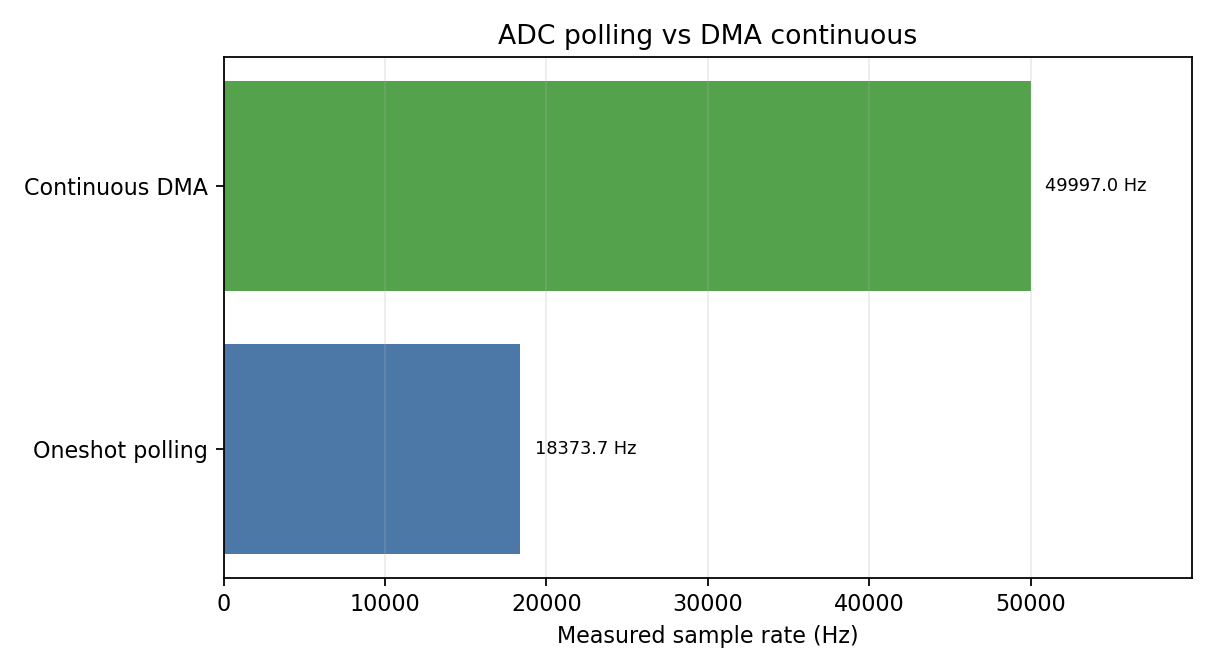
\includegraphics[width=\textwidth]{idf_dma_adc_rate_comparison.png}
    \caption{ESP-IDF 采样率}
  \end{subfigure}
  \hfill
  \begin{subfigure}{0.32\textwidth}
    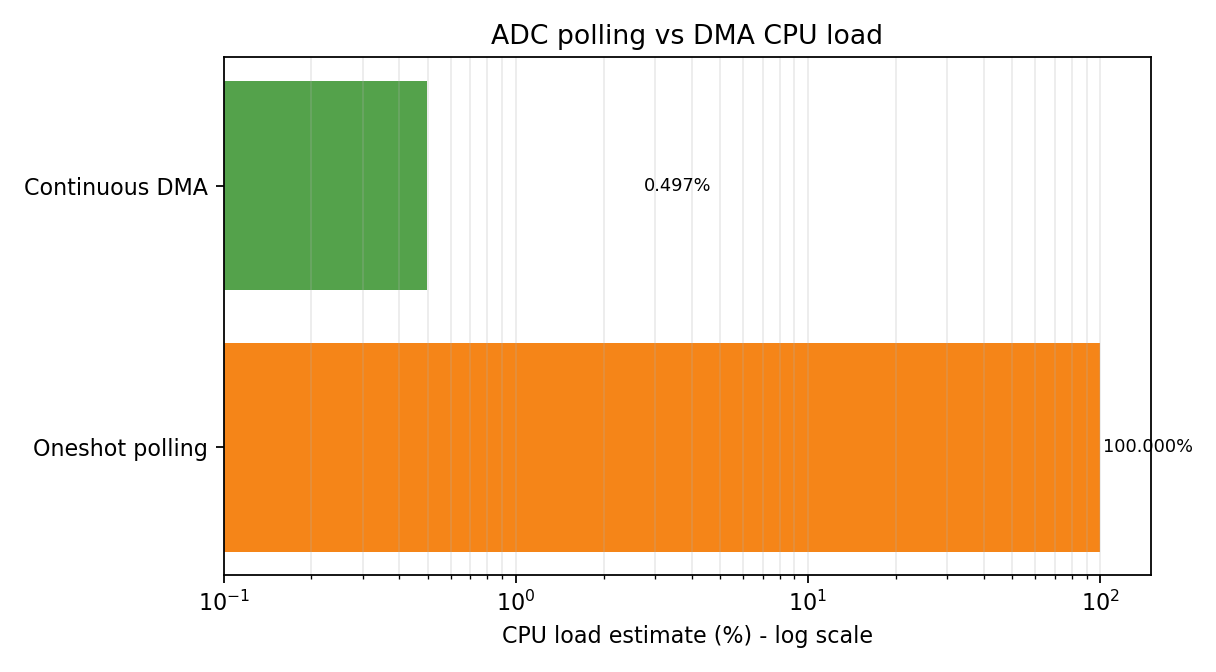
\includegraphics[width=\textwidth]{idf_dma_adc_cpu_comparison.png}
    \caption{ESP-IDF CPU 占用}
  \end{subfigure}
  \caption{ADC 采集方式对比}
\end{figure}

结果显示，查询方式虽然实现简单，但 CPU 占用接近 100\%；定时器中断可以在 1 kHz 下显著释放 CPU；DMA 双缓冲进一步将稳定采样率提高到约 50 kHz，同时将 CPU 占用降低到 0.497\%。这体现了 DMA 在高带宽数据采集中的核心优势：数据搬运由硬件完成，CPU 只需按缓冲区批量处理。

\section{中断响应延迟与 Jitter 测量}

\subsection{MicroPython 层中断测量}

实验先使用 MicroPython 在 GPIO5 输出 1 kHz 周期边沿，并在同一 GPIO 上配置上升沿 IRQ，记录 10000 次响应延迟和相邻 IRQ 间隔。

\begin{lstlisting}[language=Python,caption={GPIO 中断响应测量核心代码}]
def irq_cb(p):
    global irq_count, last_irq_us
    if not armed:
        return
    idx = irq_count
    if idx < N:
        now = time.ticks_us()
        latencies[idx] = time.ticks_diff(now, current_edge_us)
        if idx == 0:
            intervals[idx] = 0
        else:
            intervals[idx] = time.ticks_diff(now, last_irq_us)
        last_irq_us = now
        irq_count = idx + 1
\end{lstlisting}

\begin{table}[H]
\centering
\caption{MicroPython 层 10000 次中断响应统计}
\begin{tabular}{lr}
\toprule
指标 & 数值 \\
\midrule
样本数 & 10000 \\
最小响应延迟 & $29.000~\mu s$ \\
最大响应延迟 & $249.000~\mu s$ \\
平均响应延迟 & $29.723~\mu s$ \\
jitter 标准差 & $2.241~\mu s$ \\
丢包率 & 0.000\% \\
IRQ 间隔均值 & $999.972~\mu s$ \\
IRQ 间隔 jitter & $6.406~\mu s$ \\
\bottomrule
\end{tabular}
\end{table}

\begin{figure}[H]
  \centering
  \begin{subfigure}{0.48\textwidth}
    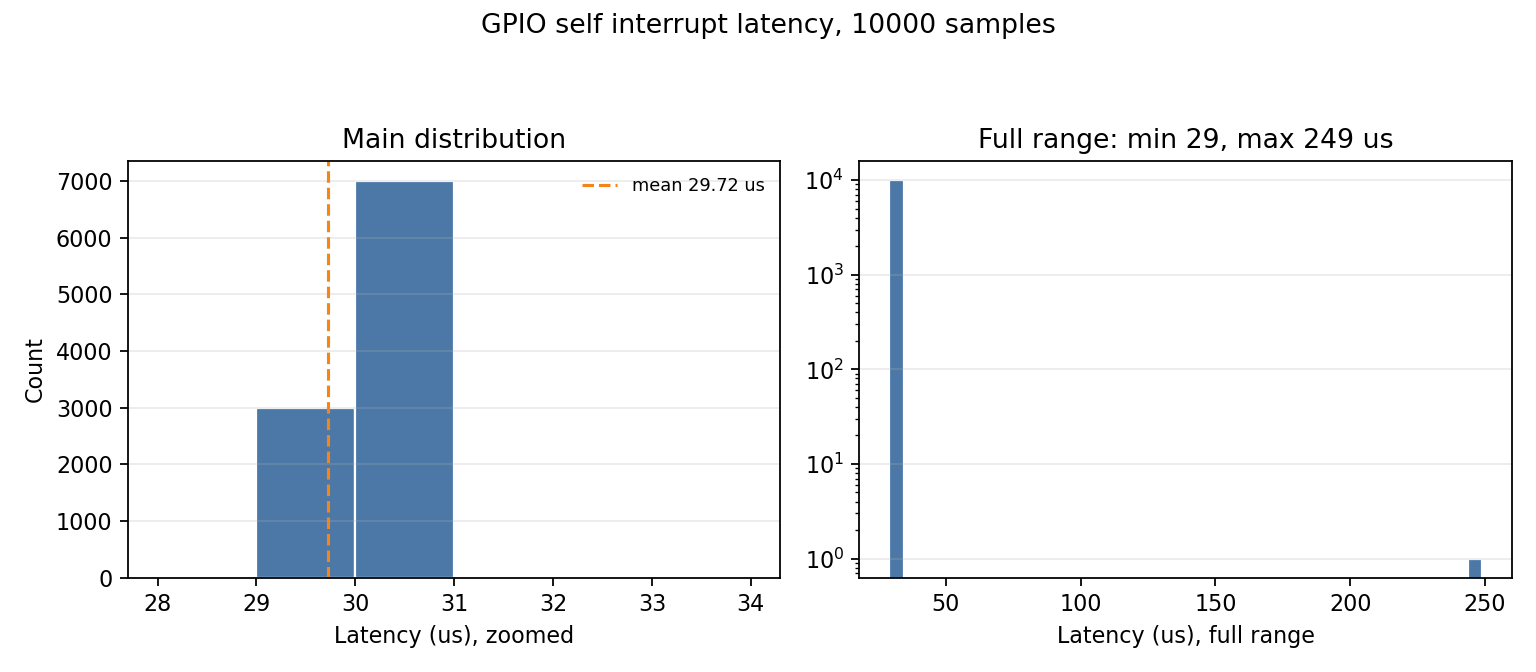
\includegraphics[width=\textwidth]{irq_latency_histogram.png}
    \caption{响应延迟直方图}
  \end{subfigure}
  \hfill
  \begin{subfigure}{0.48\textwidth}
    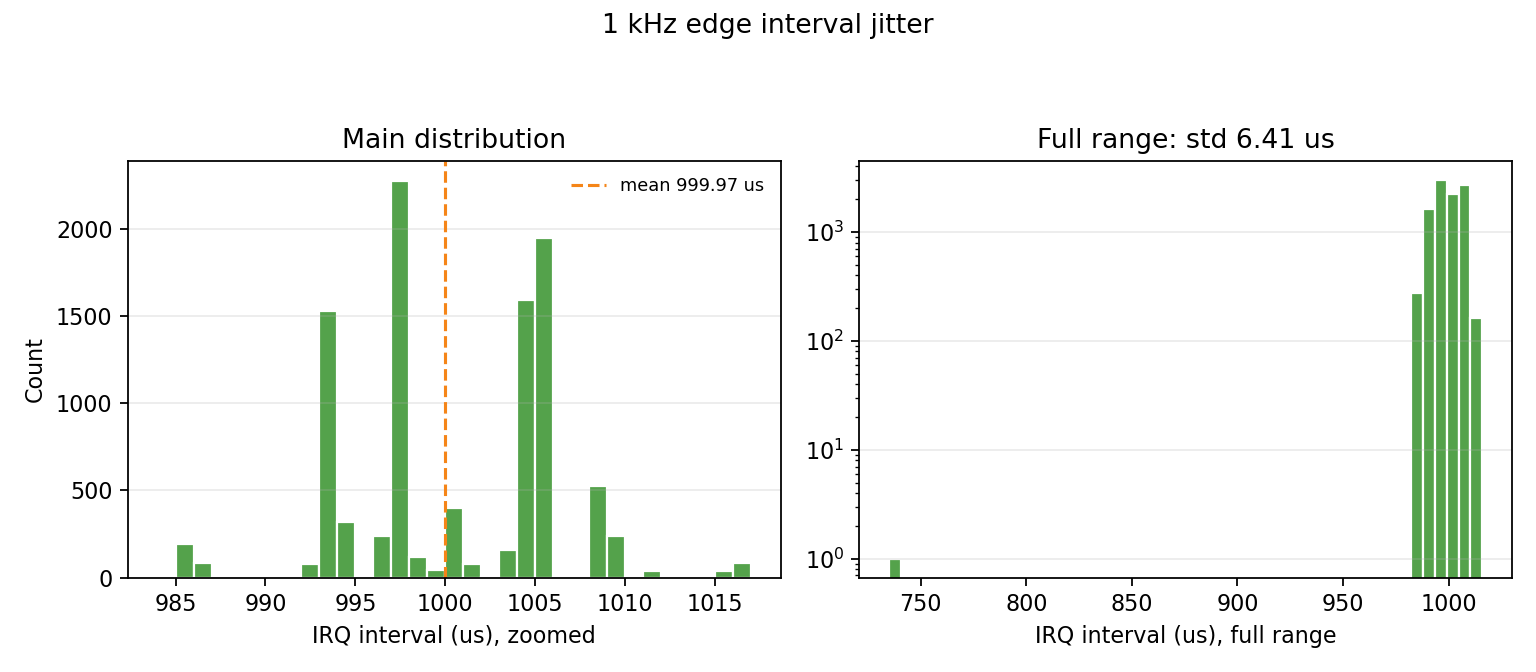
\includegraphics[width=\textwidth]{irq_interval_histogram.png}
    \caption{IRQ 间隔直方图}
  \end{subfigure}
  \caption{MicroPython 中断响应统计分布}
\end{figure}

绝大多数响应延迟集中在约 $30~\mu s$ 附近。MicroPython 结果包含解释器、回调和 \texttt{ticks\_us()} 读取开销，因此它反映的是“MicroPython 层可见响应延迟”，不是裸机 C 或硬件中断入口延迟。

\subsection{不同中断优先级补测}

ESP-IDF 补测使用 GPIO7 到 GPIO6 回环，分别配置 Level 1 和 Level 3 中断优先级，比较不同优先级下的响应延迟差异。

\begin{table}[H]
\centering
\caption{ESP-IDF 不同中断优先级响应结果}
\small
\begin{tabularx}{\textwidth}{lrrrrrrY}
\toprule
优先级 & 样本数 & 丢包率 & 最小延迟 & 最大延迟 & 平均延迟 & jitter & IRQ 间隔均值 \\
\midrule
Level 1 & 10000 & 0.000\% & $3.000~\mu s$ & $4.000~\mu s$ & $3.500~\mu s$ & $0.500~\mu s$ & $1000.000~\mu s$ \\
Level 3 & 10000 & 0.000\% & $3.000~\mu s$ & $4.000~\mu s$ & $3.500~\mu s$ & $0.500~\mu s$ & $1000.000~\mu s$ \\
\bottomrule
\end{tabularx}
\end{table}

\begin{figure}[H]
  \centering
  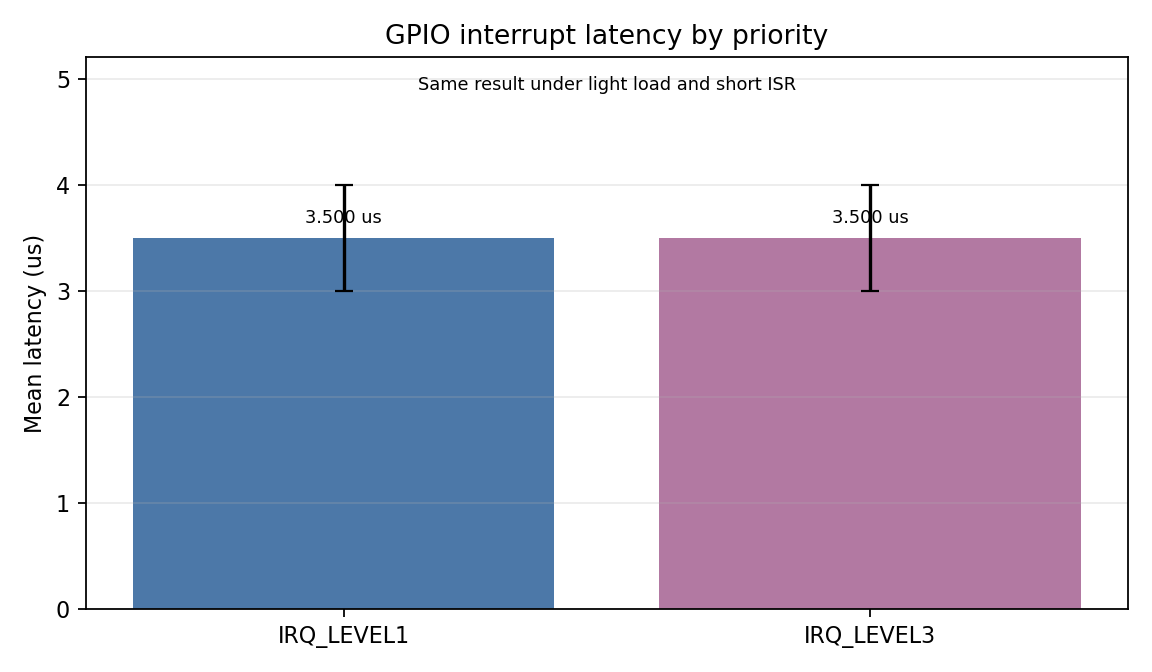
\includegraphics[width=0.76\textwidth]{idf_irq_priority_latency.png}
  \caption{ESP-IDF 不同中断优先级延迟对比}
\end{figure}

在本次测试负载较低、ISR 很短、没有额外高优先级任务抢占的条件下，Level 1 与 Level 3 的平均延迟均为 $3.500~\mu s$，差异不明显。中断优先级的影响通常需要在存在竞争中断、长时间临界区或高优先级任务抢占时才更容易体现。

\section{时间戳精度测量}

时间戳测量脚本每秒输出一次 ESP32 \texttt{ticks\_ms()} 和 \texttt{ticks\_us()}，PC 端捕获脚本同步记录 \texttt{time.time\_ns()}，再计算 ESP32 相对 PC 标准时间的漂移。

\begin{lstlisting}[language=Python,caption={板端时间戳输出核心代码}]
PERIOD_MS = 1000
DEFAULT_SAMPLES = 3600

freq = machine.freq()
start = time.ticks_ms()
next_t = start
for i in range(DEFAULT_SAMPLES + 1):
    while time.ticks_diff(time.ticks_ms(), next_t) < 0:
        time.sleep_ms(5)
    print("%d,%d,%d,%d" % (i, time.ticks_ms(), time.ticks_us(), freq))
    next_t = time.ticks_add(next_t, PERIOD_MS)
\end{lstlisting}

本次采集共获得 3601 条板端时间戳记录，PC 参考时长 3599.840 s，1 小时末端偏差约 158.536 ms，折算晶振或计时链路频率误差约 44.040 ppm。ppm 计算方式为：

\[
\mathrm{ppm} = \frac{T_{\mathrm{ESP32}} - T_{\mathrm{PC}}}{T_{\mathrm{PC}}} \times 10^6
\]

\begin{figure}[H]
  \centering
  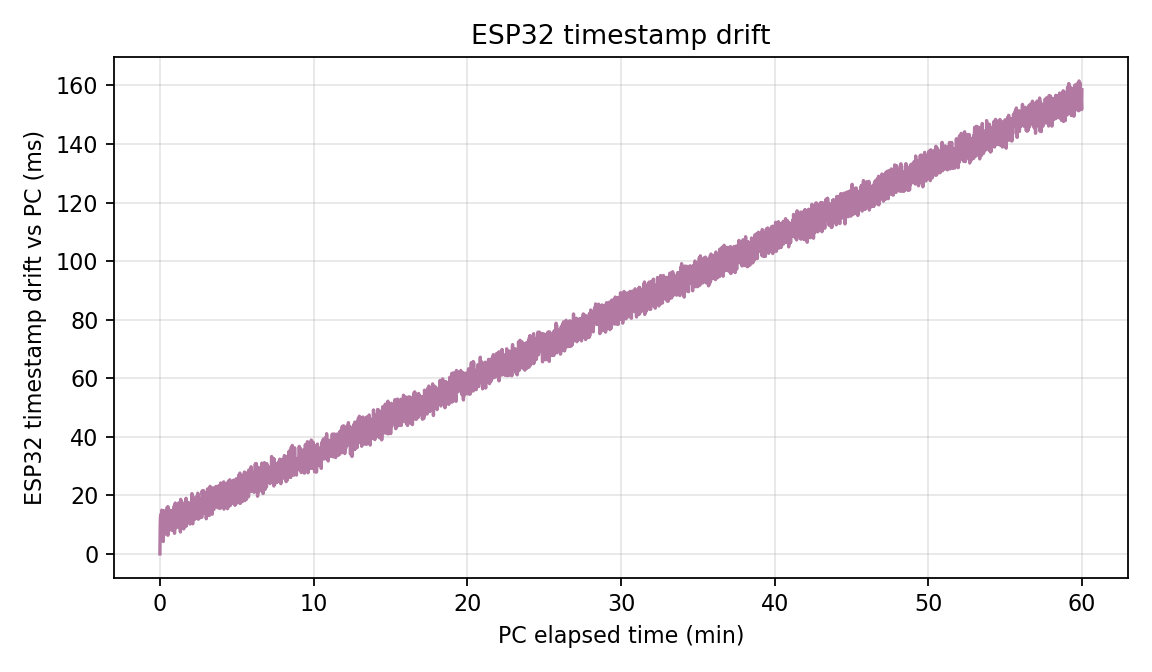
\includegraphics[width=0.82\textwidth]{timestamp_drift_curve.png}
  \caption{ESP32 时间戳相对 PC 时间漂移曲线}
\end{figure}

PC 时间并不是实验室级标准时钟，因此本实验 ppm 反映的是 ESP32 MicroPython 时间戳链路相对 PC 系统时钟的偏差，包含串口输出、PC 调度和系统时钟误差。若需要更严格结果，应使用 GPSDO、频率计或逻辑分析仪作为基准。

\section{结果分析}

\begin{enumerate}[label=\arabic*.]
  \item GPIO 和 PWM 可直接由 ESP32-S3 板内外设完成。GPIO48 板载 RGB LED 能直观验证输出功能，GPIO5 PWM 回接 GPIO4 后可通过 ADC 统计占空比。
  \item 查询方式实现简单，但在高频采样时 CPU 占用接近 100\%，不适合复杂实时任务。
  \item 定时器中断方式能稳定实现 1 kHz 周期采样，CPU 占用明显低于忙等待查询方式，是中低速周期采集的合理方案。
  \item 中断响应延迟的 jitter 来自解释器调度、回调执行时间、\texttt{ticks\_us()} 时间戳读取开销和串口或系统后台任务影响。MicroPython 层测得约几十微秒量级，适合课程级实时性认识；ESP-IDF 裸机 ISR 补测可把可见延迟降低到约 $3.5~\mu s$。
  \item DMA 双缓冲适用于更高带宽 ADC 采集。其核心优势是 ADC 数据搬运由 DMA 完成，CPU 只在缓冲区事件中批量处理数据，从而降低中断频率和 CPU 负载。
  \item 在低负载、短 ISR 条件下，Level 1 与 Level 3 中断优先级延迟结果相同，说明优先级差异主要在中断竞争、长临界区或高优先级任务抢占时体现。
  \item 时间戳漂移 ppm 可用于理解晶振误差对同步系统的影响。例如 100 ppm 误差会造成每秒 $100~\mu s$、每小时约 360 ms 的累积偏差，因此长时间同步需要校时或频率补偿。
\end{enumerate}

\section{实验任务逐项核对}

\begin{longtable}{>{\raggedright\arraybackslash}p{0.25\textwidth}>{\raggedright\arraybackslash}p{0.15\textwidth}>{\raggedright\arraybackslash}p{0.50\textwidth}}
\caption{实验任务完成情况核对}\\
\toprule
实验要求 & 完成情况 & 证据文件或结果 \\
\midrule
\endfirsthead
\toprule
实验要求 & 完成情况 & 证据文件或结果 \\
\midrule
\endhead
GPIO 输出控制 LED & 已完成 & GPIO48 板载 RGB 闪烁，\path{code/01_gpio_pwm_adc_timer_demo.py} \\
PWM 呼吸灯或输出 & 已完成 & GPIO48 亮度渐变，GPIO5 PWM 输出 \\
ADC 采集 & 已完成 & \path{data/pwm_adc_loopback_stats.csv}，GPIO5 到 GPIO4 板内回环 \\
1 kHz 定时器中断采集 & 已完成 & \path{data/polling_vs_timer_adc_smoke.csv} \\
查询与中断 CPU 占用对比 & 已完成 & 查询 100\%，定时器约 8.494\% \\
DMA 双缓冲 ADC & 已完成 & ESP-IDF 连续 ADC DMA：49997.0 Hz，CPU 0.497\% \\
10000 次中断响应统计 & 已完成 & \path{data/self_irq_latency_10000.csv}，平均 $29.723~\mu s$ \\
时间戳精度测量 & 已完成 & 1 小时时间戳数据与漂移曲线 \\
不同中断优先级对比（选做） & 已完成 & Level 1 与 Level 3 各 10000 次，平均延迟均为 $3.500~\mu s$ \\
\bottomrule
\end{longtable}

\section{提交文件说明}

\begin{table}[H]
\centering
\caption{提交包文件说明}
\begin{tabularx}{\textwidth}{lY}
\toprule
文件或目录 & 内容 \\
\midrule
\texttt{report.md} & 原始 Markdown 实验报告 \\
\texttt{index.html} & 可直接浏览的网页报告 \\
\texttt{data/} & 原始数据、清洗数据和统计 JSON \\
\texttt{assets/} & PWM-ADC、CPU 占用、DMA 采样率、中断延迟、优先级对比、时间漂移图 \\
\texttt{code/} & MicroPython 板端脚本和 ESP-IDF DMA/IRQ 补测工程 \\
\texttt{README.md} & 提交包说明 \\
\bottomrule
\end{tabularx}
\end{table}

\section{参考资料}

\begin{enumerate}[label={[\arabic*]}]
  \item MicroPython ESP32 Quick Reference: \url{https://docs.micropython.org/en/latest/esp32/quickref.html}
  \item MicroPython \texttt{machine} 模块文档: \url{https://docs.micropython.org/en/latest/library/machine.html}
  \item Espressif ESP-IDF ADC Continuous Mode Driver Programming Guide: \url{https://docs.espressif.com/projects/esp-idf/en/latest/esp32/api-reference/peripherals/adc_continuous.html}
\end{enumerate}

\end{document}
